\documentclass[12pt,a4paper,twoside,openany]{book}
\usepackage[italian]{babel}
\renewcommand{\baselinestretch}{1.5} 
\usepackage[]{frontespizio}
\usepackage[autostyle,italian=guillemets,]{csquotes}
\usepackage[bibstyle=authortitle,citestyle=verbose-trad1,backend=biber,style=numeric]{biblatex}
\addbibresource{tesi.bib}
\usepackage[]{hyperref}

\begin{document}

\begin{frontespizio}
\Rientro {1.5cm}
\Margini {1.5cm}{1.5cm}{1.5cm}{1cm}
\Universita {Modena e Reggio Emilia}
%\Logo [1.5cm]{immagini/UNIMORE.jpg}
\Dipartimento {Ingegneria "Enzo Ferrari"}
\Corso [Laurea]{Ingegneria Informatica}
\Annoaccademico {2020-2021}
\Titoletto {Prova Finale}
\Titolo {Sviluppo di un'applicazione che integra algoritmi di machine learning con Apache PredictionIO}
\Candidato [132097]{Francesco Baraldi}
\Relatore {Prof. Francesco Guerra}
%\Correlatore{da inserire}
\end{frontespizio}

%\newpage
%\begin{flushright}
%\null\vspace{\stretch{1}}
%\textit{All'unione di Shiva e Parvati che rende feconda la distruzione.}
%\vspace{\stretch{2}}\null
%\end{flushright}

\tableofcontents
\listoffigures

\chapter{Introduzione}\label{c:introduzione}

Il machine learning è un sottoinsieme dell'intelligenza artificiale che si occupa di creare sistemi che apprendono e migliorano le loro performance sulla base dei dati che utilizzano. L'idea alla base è che i sistemi possono eseguire dei compiti specifici senza essere programmati per farlo,  imparando dai dati e identificando dei modelli all'interno di essi.

La crescita esponenziale del volume dei dati prodotti ha permesso un grande sviluppo di algoritmi di machine learning,  che al giorno d'oggi hanno raggiunto una diffusione capillare all'interno dei sistemi più utilizzati,  dalle applicazioni web e mobile,  agli assistenti virtuali fino all'assistenza alla guida per le automobili.  In particolare nel campo del marketing,  i siti web di e-commerce utilizzano il machine learning per consigliare agli utenti dei prodotti che potrebbero interessare maggiormante l'acquirente sulla base degli ultimi acquisti o delle ricerche fatte. Nel campo finanziario invece è possibile identificare delle opportunità di investimento studiando i dati di mercato di molte aziende, aiutando così gli investitori a fare investimenti corretti.

Sviluppare applicazioni, che siano desktop, mobile o web app, che utilizzino algoritmi di apprendimento automatico però non è banale, perchè richiede conoscenza di data analysis e di machine learning per poter implementare un algoritmo all'interno della propria applicazione. Esiste però la possibilità di sfruttare algoritmi di machine learning in modo più agevole e veloce per gli sviluppatori, sviluppando le proprie applicazioni in modo che debbano solo interfacciarsi con dei servizi web, i quali gestiranno tutta la parte di machine learning e si occuperanno di fornire le predizioni richieste. Questo è possibile grazie al software Apache PredictionIO che permette di creare dei servizi web con i quali qualsiasi applicazione può interagire tramite richieste HTTP e usare qualsiasi algoritmo di machine learning in modo più facile e veloce rispetto a come sarebbe integrarlo direttamente all'interno dell'applicazione. Grazie a un software come PredictionIO quindi il machine learning diventa accessibile a qualsiasi sviluppatore e non solo ai data scientist.

Ho quindi deciso di sviluppare un'applicazione desktop per la valutazione di aziende in ambito finanziario che permetta agli utenti di avere supporto per gli investimenti. Questa applicazione si interfaccia con il software Apache PredictionIO per avere valutazioni sul futuro andamento dell'azienda e avere consigli su altre aziende simili, sulla base del profilo  e degli attuali interessi di un utente.

Il documento prosegue con il capitolo \ref{c:predictionio}, nel quale viene introdotto e spiegato il funzionamento di Apache PredictionIO, approfondendo la sua architettura e le sue componenti, spiegando infine una possibile via per l'installazione. Nel capitolo \ref{c:applicazione} viene spiegato come è stata sviluppata l'applicazione, le sue funzionalità e la sua struttura, spiegando infine come si integra con PredictionIO. Nel capitolo \ref{c:conclusione} si traggono le conclusioni facendo delle considerazioni finali.
\chapter{PredictionIO}\label{c:predictionio}

Apache PredictionIO è un software open source che permettere di sviluppare dei server per il machine learning per qualsiasi task, in particolare è possibile creare degli engines, o modificarne di già esistenti per adattarli alle proprie esigenze, per gestire uno o più algoritmi di machine learning. Le sue funzionalità sono:
\begin{itemize}
\item implementare degli engines ed effetturane il deploy come web service,
\item interrogare un engine con delle query dinamiche e ricevere risposte in real-time,
\item valutare e modificare un engine in modo dinamico,
\item creare un proprio modello di machine learning e implementarlo in un nuovo engine.
\end{itemize}
Da settembre 2020 Apache PreditcionIO è stato messo "nell'attico" da Apache, il che significa che non sarà più supportato e aggiornato da chi l'ha sviluppato, ma è ancora perfettamente funzionante e ho scelto di utilizzarlo perchè credo che le sue funzionalità portino valore nel software development e consentano agli sviluppatori software di integrare algoritmi di machine learning in modo agevole e veloce.

\section{Architettura di PredictionIO}
Apache PredictionIO si integra con applicazioni mobile, web o desktop, le quali possono inviare dei dati all'\textbf{event server}, il quale conserverà i dati, appoggiandosi al database HBase di Apache, i quali saranno poi utilizzati per l'addestramento del modello. L'applicazione potrà mandare dati all'event server in qualsiasi momento, anche dopo il deploy e l'engine di PredictionIO potrà aggiornarsi in modo dinamico effettuando un continuo addestramento che gli permetterà di adattarsi ai dati che gli utenti dell'applicazione continueranno a produrre.

\begin{figure}[!h]
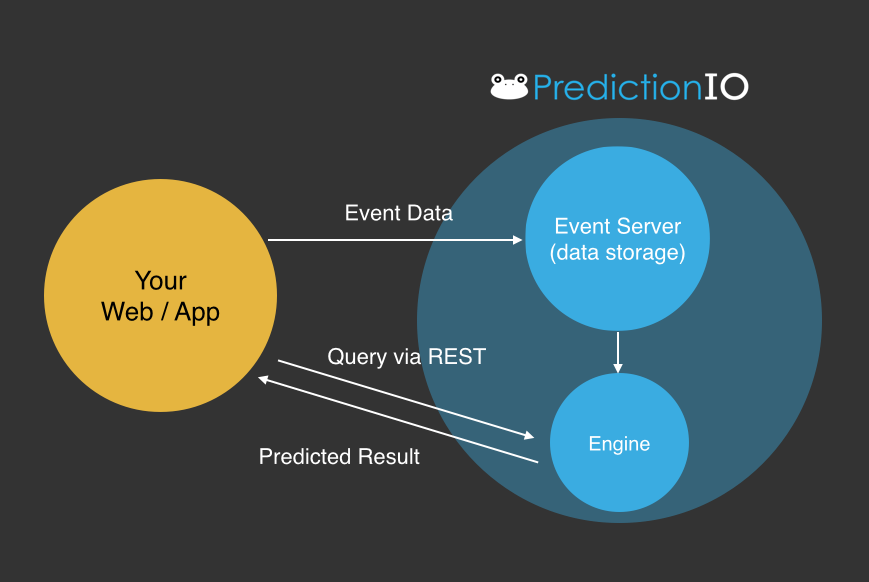
\includegraphics[width=1.0\textwidth]{immagini/app_integration.png}
\caption{Architettura di PredictionIO \cite{sitopredictionio}}
\label{fig:app_integration}
\end{figure}

L'engine o gli engines implementati per l'applicazione si interfacceranno con l'event server per leggere i dati e fare l'addestramento, inoltre potranno ricevere delle richieste tramite query REST dall'app e risponderanno in real-time fornendo la previsione.

\section{Event Server}
L'event server è la componente che memorizza i dati inviati dall'applicazione. Questi dati sono salvati in un database, in particolare viene usato HBase, e verranno mandati al modello nel momento dell'addestramento. I dati vengono salvati con uno stile \textit{event-based}: l'applicazione manda "eventi" che avranno determinate caratteristiche e attributi a seconda del task del modello. Ogni evento ha un "entityType" che rappresenta il tipo di entità che quell'evento rappresenta e può essere personalizzato dallo sviluppatore a seconda dei propri dati (ad esempio "user", "item", "product"...); un "entityId" per identificare l'entità di quell'evento, e altri attributi definiti dallo sviluppatore per descrivere le entità che devono essere rappresentate. Infine gli eventi possono essere di tre tipi:

\begin{itemize}
\item \textbf{"\$set"}: per inserire una nuova entità o modificare gli attributi di una già esistente.
\item \textbf{"\$unset"}: per mantenere un'entità in memoria ma considerarla come se fosse eliminata.
\item \textbf{"\$delete"}: per eliminare un'entità.
\end{itemize}

\newpage

\begin{figure}[!ht]
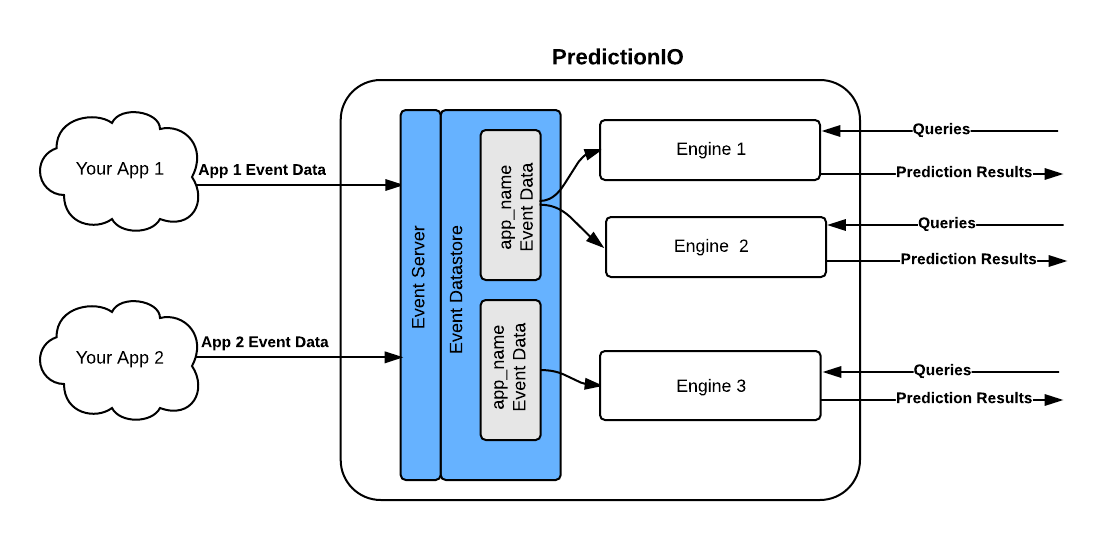
\includegraphics[width=1.0\textwidth]{immagini/eventserver.png}
\caption{Event Server \cite{sitopredictionio}}
\label{fig:eventserver}
\end{figure}

L'event server deve essere attivato anch'esso come servizio web prima di poter ricevere dei dati e prima di mandarli al modello per l'addestramento. Con il comando \verb+pio eventserver+ l'event server viene avviato e sarà disponibile di default all'indirizzo http://localhost:7070.

L'event server può contenere i dati di più engines quindi è necessario specificare a quale modello ogni dato è riferito. Per farlo si creano, con il comando \verb+pio app new myapp+, delle \textit{pio app} relative ad un solo engine, ogni app avrà come identificatore una \textit{access key} che sarà specificata nei dati che vengono mandati all'event server. In questo modo quando sarà il momento di addestrare un modello l'event server fornirà i dati solo relativi all'access key di quell'engine.

\section{Engines come servizi web}
Un engine è un'identità logica che rappresenta un algoritmo di machine learning per un determinato task, può interagire con una sola applicazione ed è specifico per un determinato task, mentre un'applicazione può interagire con più engines. Gli engine possono essere di diverso tipo:
\begin{itemize}
\item raccomandazione: per task relativi a "raccomandare" prodotti sulla base di preferenze e gusti di un utente,
\item classificazione: per task relativi a classificare un determinato target, si basa sui principali algoritmi di classificazione,
\item regressione: per task per valutare un target con un valore continuo, quindi si basa sugli algoritmi di regressione.
\end{itemize}

Le funzioni di un engine quindi sono quelle di leggere i dati dall'event server per l'addestramento del modello che l'engine rappresenta, dopodichè viene fatto il deploy come servizio web e infine deve rispondere alle richieste ricevute dall'applicazione facendo predizioni.

\subsection{DASE}
Un engine è strutturato con un'architettura che prende il nome di \textbf{DASE}, acronimo di \textbf{D}ata Source and Preparator, \textbf{A}lgorithm, \textbf{S}erving e \textbf{E}valuation Metrics. 
\begin{itemize}
\item \textbf{Data Source e Preparator}: la componente di data source prende i dati in input e li trasforma nel formato desiderato dal modello di machine learning che viene utlizzato; mentre la componente di data preparator prende i dati processati dal data source e li manda in input all'algoritmo per l'addestramento.
\item \textbf{Algorithm}: la componente algorithm include l'algoritmo di machine learning vero e proprio, con il settaggio dei parametri e determina come il modello è costruito. La componente algorithm si basa sulla piattaforma Apache Spark, in particolare sulla libreria Spark's MLLib (machine learning library), che gestirà tutta la parte di addestramento dell'algoritmo scelto.
\item \textbf{Serving}: la componente di serving ha il compito di ricevere in input le richieste dell'applicazione, mandarle al modello e rispondere con il risultato predetto.
\item \textbf{Evaluation Metrics}: la componente di evaluation valuta le performance del modello e ne dà un risultato numerico, può essere usata quindi per fare comparazioni tra diversi algoritmi.
\end{itemize}

\begin{figure}[!h]
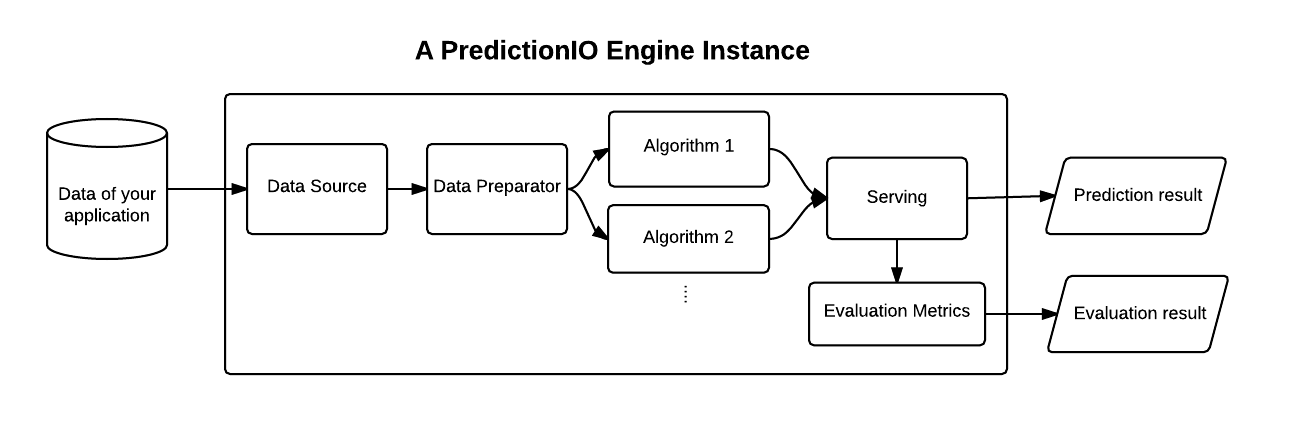
\includegraphics[width=1.0\textwidth]{immagini/dase.png}
\caption{Architettura DASE \cite{sitopredictionio}}
\label{fig:dase}
\end{figure}

\subsection{Addestramento e deploy}
Un engine quindi consiste nelle varie componenti DASE che sono implementate in un proggetto nel linguaggio Scala, un linguaggio orientato agli oggetti la cui compilazione produce bytecode java eseguibile su una Java Virtual Machine. Sono disponibili molti engine template per i vari tipi disponibili, in modo che uno sviluppatore possa partire da uno di questi template già pronti, con le vari componenti DASE già implementate e andare a modificare le componenti solo per adattarle al proprio task specifico, altrimenti è anche possibile svilupparlo da zero.

Una volta implementato un engine, è necessario eseguire una serie di operazioni per renderlo operativo:
\begin{itemize}
\item \textbf{build del progetto}: con il comando \verb+pio build+ viene eseguito il build del progetto,
\item \textbf{training}: con il comando \verb+pio train+ l'engine legge i dati relativi al suo modello dall'event server ed esegure l'addestramento dell'algoritmo,
\item \textbf{deploy come servizio web}: dopo aver correttamente addestrato il modello è possibile eseguirne il deploy con il comando \\ \verb+pio deploy --port 8000+, in questo modo il modello sarà disponibile come servizio web alla porta specificata nel comando, in questo caso alla porta 8000.
\end{itemize}

\begin{figure}[!h]
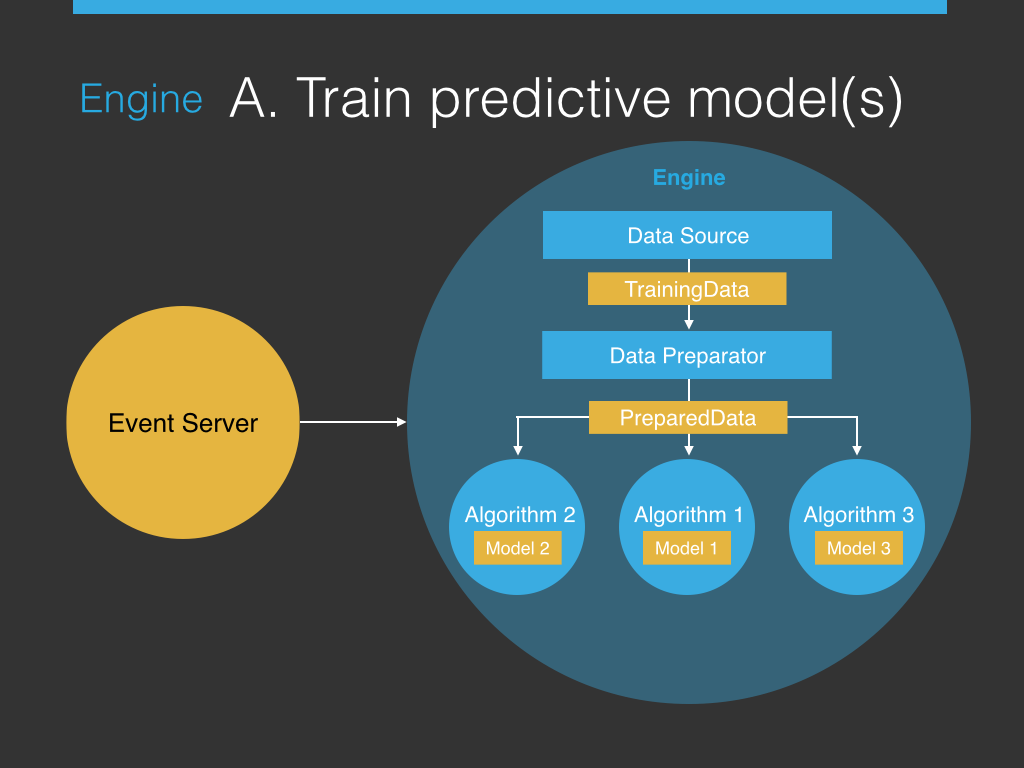
\includegraphics[width=0.8\textwidth]{immagini/training.png}
\caption{Addestramento \cite{sitopredictionio}}
\label{fig:training}
\end{figure}

Dopo aver eseguito questi passaggi è possibile fare richieste al modello con query REST all'indirizzo http://localhost:8000 (nel caso l'engine sia operativo sulla macchina locale). L'applicazione che dovrà interagire con il modello potrà sfruttare le API's di PredictionIO disponibili per i principali linguaggi di programmazione(Java, Python, Ruby, PHP...).

\begin{figure}[!h]
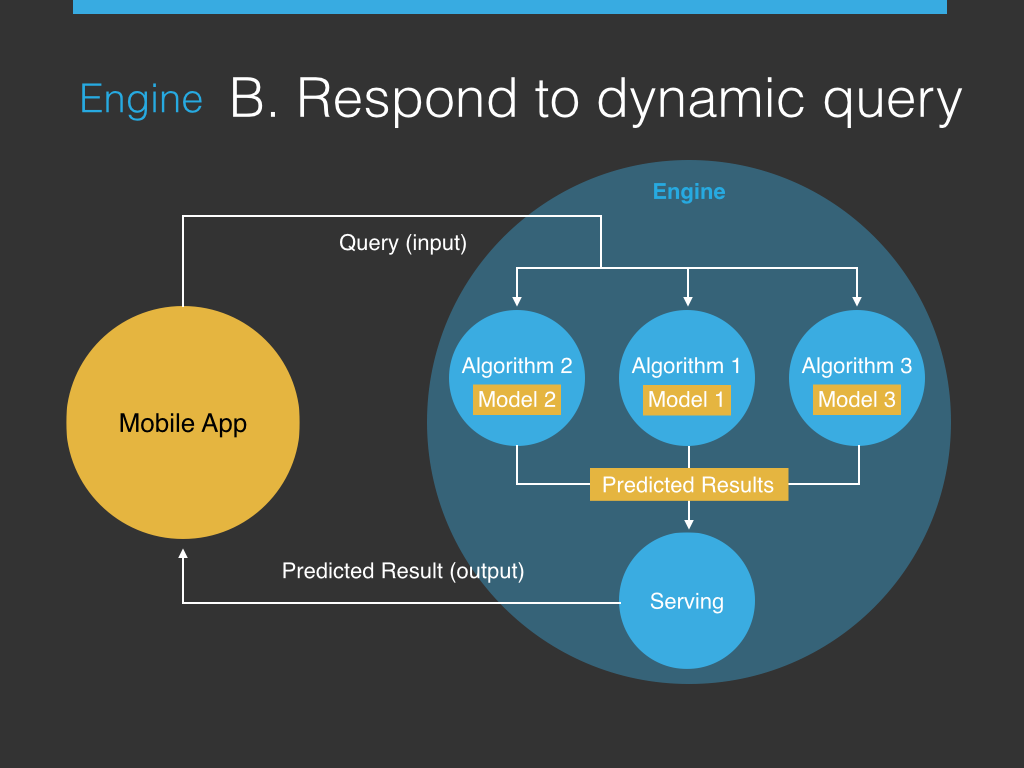
\includegraphics[width=0.8\textwidth]{immagini/deploy.png}
\caption{Interazione app-engine \cite{sitopredictionio}}
\label{fig:deploy}
\end{figure}

\newpage

\section{Installazione con Docker}
Il software PredictionIO può essere installato in modo nativo su una qualsiasi macchina UNIX. In questo caso però è necessario gestire manualmente tutte le numerose dipendenze e potrebbero sorgere problemi di compatibilità. Per lo svolgimento di questo elaborato è stato quindi scelto di installare il software utilizzando Docker.

\subsection{Docker}
Docker consente di automatizzare il deploy di software all'interno di \textbf{container} software, aggiungendo un livello di astrazione grazie alla virtualizzazione del sistema operativo Linux. Lo scopo di Docker quindi è quello di fornire dei "package" che contengono un software installato con tutte le sue dipendenze in modo da essere già pronto per il deploy, e quindi facilmente utilizzabile. A differenza delle classiche macchine virtuali Docker fornisce container più leggeri e più isolati, che possono essere installati a prescindere dalla macchina host che li ospiterà garantendo forte granularità e portabilità.

\subsection{PreditionIO con Docker}
PredictionIO fornisce piena compatibilità con Docker ed è facilmente installabile utilizzando il container già disponibile. Una volta scaricato il software open source di PredictionIO si può installare l'immagine Docker facilmente con il comando \verb+docker build -t predictionio/pio pio+, dove il software di PredictionIO è nella directory chiamata \verb+predictionio+ (l'unico requisito è avere Docker installato e funzionante sulla propria macchina). Dopodiché dalla sottocartella \verb+predictionio/docker+ è possibile avviare PredictionIO e utilizzare i comandi già visti prima per creare engine ed eseguire i vari passaggi, con l'unica differenza di usare il comando \verb+pio-docker+ al posto di \verb+pio+.
\chapter{Sviluppo applicazione}\label{c:applicazione}

L'applicazione che è stata sviluppata ha lo scopo di fornire un supporto per gli utenti interessati agli investimenti in aziende e start up, usando algoritmi di machine learning per predire l'andamento futuro di un'azienda, sulla base di alcuni dati rappresentativi dell'azienda specifica. 

È stato deciso di sviluppare un'applicazione desktop in linguaggio Python perchè il più adatto per la gestione dei dati e la loro manipolazione prima di essere usati per algoritmi di machine learning, e data la piena compatibilità con le API di PredictionIO per l'interazione con l'event server e i vari engines. Infatti la parte di machine learning è gestita interamente da PredictionIO. Mentre per l'interfaccia grafica è stata usata la libreria TKinter di Python, la libreria grafica standard per questo linguaggio.

Di seguito sarà illustrato come è stata sviluppata l'applicazione, come è stato usato PredictionIO e come si integra con l'applicazione.

\section{Funzionalità e scopo}
L'applicazione sviluppata consente di creare un account personale inserendo i propri dati, con il quale sarà poi possibile cercare aziende presenti nell'applicazione e vederne i principali dati, salvare nei preferiti quelle che interessano di più e poter fare una previsione sull'andamento futuro dell'azienda e quindi sulla convenienza di investimento. 

\begin{figure}[!h]
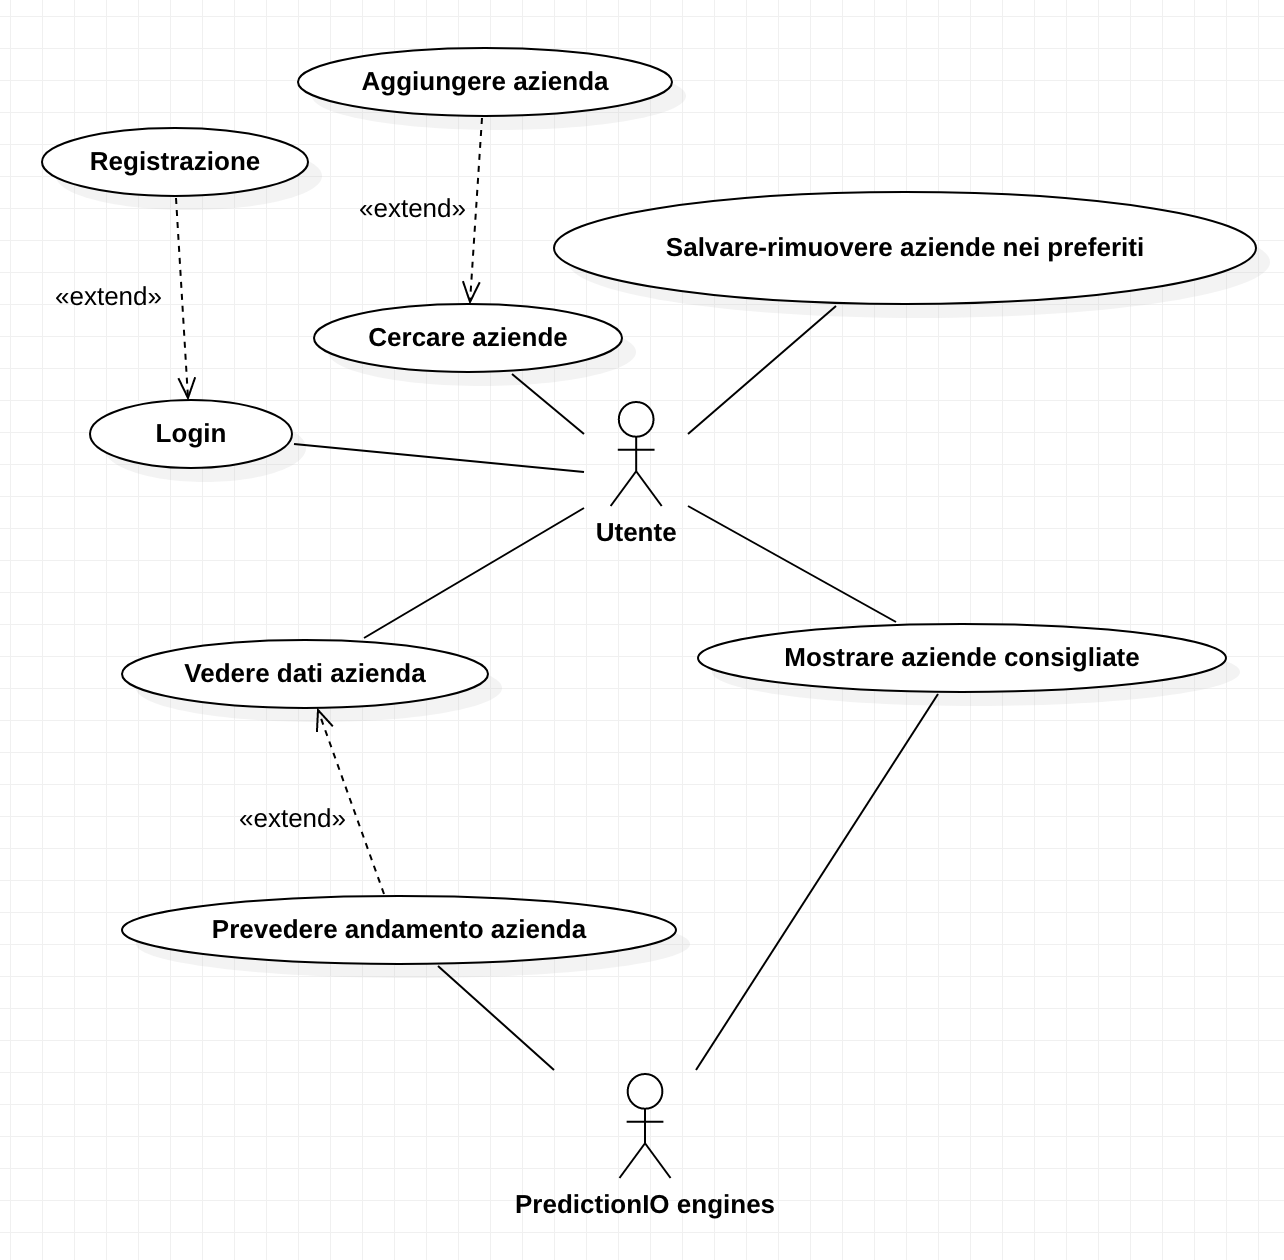
\includegraphics[width=1.0\textwidth]{immagini/usecase.png}
\caption{Use Case Diagram}
\label{fig:usecase}
\end{figure}

\section{Struttura dell'applicazione}
L'applicazione si compone di diversi moduli rappresentati da classi Python. Alcuni moduli rappresentano delle schermate dell'applicazione, ognuna con una funzionalità diversa:
\begin{itemize}
\item \textbf{Schermata di login}: è la prima schermata mostrata quando si avvia l'applicazione e semplicemente consente di effettuare il login inserendo \textit{username} e \textit{password}.
\item \textbf{Schermata di registrazione}: se non si ha già un account, dalla schermata di login è possibile spostarsi nella schermata di registrazione per creare un nuovo account inserendo i propri dati.
\item \textbf{Schermata di home page}: è la schermata principale che compare quando si effettua il login e nella quale sono presenti tre sezioni principali:
\begin{itemize}
\item \textbf{Preferiti}: nella quale vengono mostrate le aziende salvate come preferite da quell'utente.
\item \textbf{Consigliati}: nella quale vengono mostrate delle aziende consigliate in base alle preferenze di quell'utente. Questa lista viene creata usando un algoritmo di machine learning di recommendation, implementato in un engine di PredictionIO (si veda  \ref{subsubsec:racc}).
\item \textbf{Ricerca}: nella quale si possono effettuare delle ricerche specificando il nome dell'azienda che si vuole trovare.
\end{itemize}
\item \textbf{Profilo}: è la schermata nella quale è possibile modificare i dati del proprio account, come username, nome e cognome, o fare la reimpostazione della password.
\item \textbf{Azienda}: è la schermata che descrive l'azienda, mostrando i dati principali e nella quale è possibile salvare nei preferiti quell'azienda, o toglierla dai preferiti nel caso fosse già salvata. Inoltre è possibile richiedere una previsione sul futuro andamento dell'azienda con dei relativi consigli sull'investimento, questo è possibile grazie a un algoritmo di machine learning di classificazione, il RandomForest, implementato in un engine di PredictionIO (si veda \ref{subsubsec:class}).
\item \textbf{Inserimento azienda}: se un'azienda non è presente e non viene trovata con una ricerca è possibile aggiungerla inserendo i dati richiesti.
\end{itemize}

Altri moduli fondamentali sono la \textbf{Main Page}, che ha il compito di gestire le varie schermate e le transizioni tra esse. Il \textbf{DBManager} che gestisce il database, consentendo di modificare i dati aggiungendo o modificando utenti nella fase di iscrizione o quando si modificano i propri dati. Il \textbf{Predictor} infine è il modulo che gestisce le parti di machine learning e quindi è dove è implementata l'integrazione con gli engines di PredictionIO.

Le classi che rappresentano i moduli di cui sopra sono rappresentate dal seguente class diagram.

\newpage

\begin{figure}[!h]
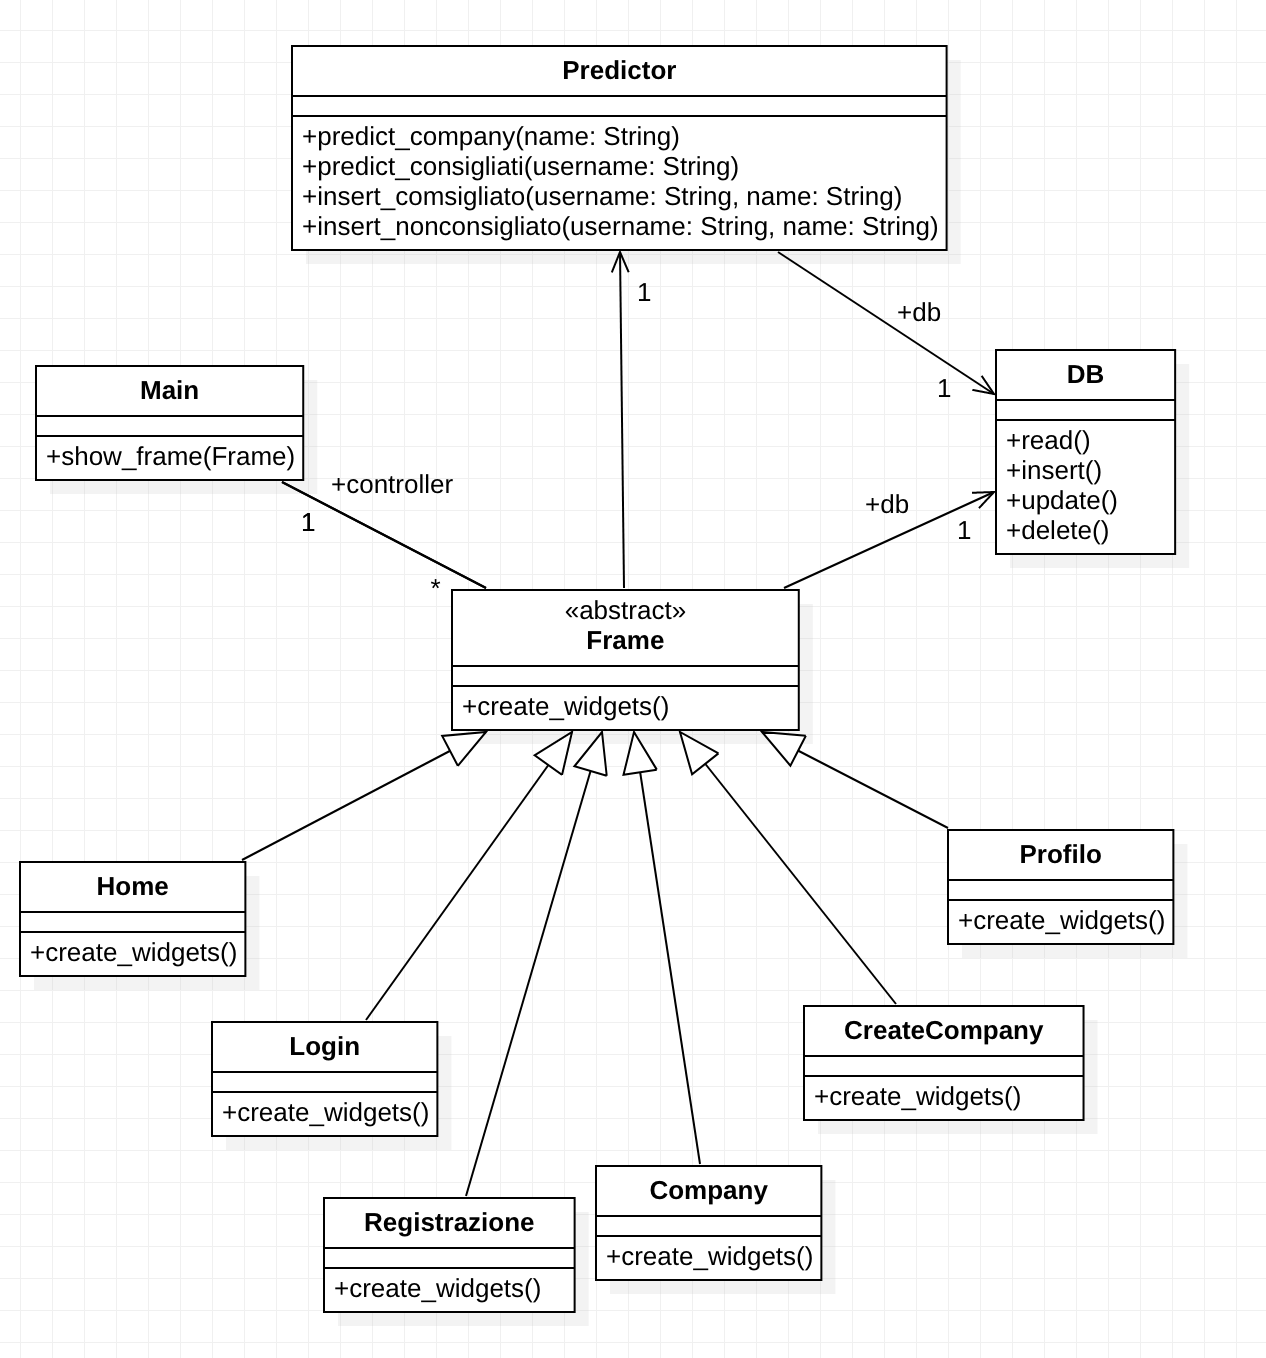
\includegraphics[width=1.0\textwidth]{immagini/classdiagram.png}
\caption{Class Diagram}
\label{fig:classdiagram}
\end{figure}

In particolare la classe \textbf{Frame} è la classe madre di tutti i moduli che rappresentano delle schermate, ogni implementazione concreta sovrascriverà il metodo \verb+create_widgets()+ che ha lo scopo di creare gli elementi visivi presenti e posizionarli sulla schermata di riferimento con le dovute dimensioni e distanze tra essi. Di seguito un esempio di metodo \verb+create_widgets()+ della classe LoginPage, che rappresenta la schermata di login. 

\begin{figure}[!h]
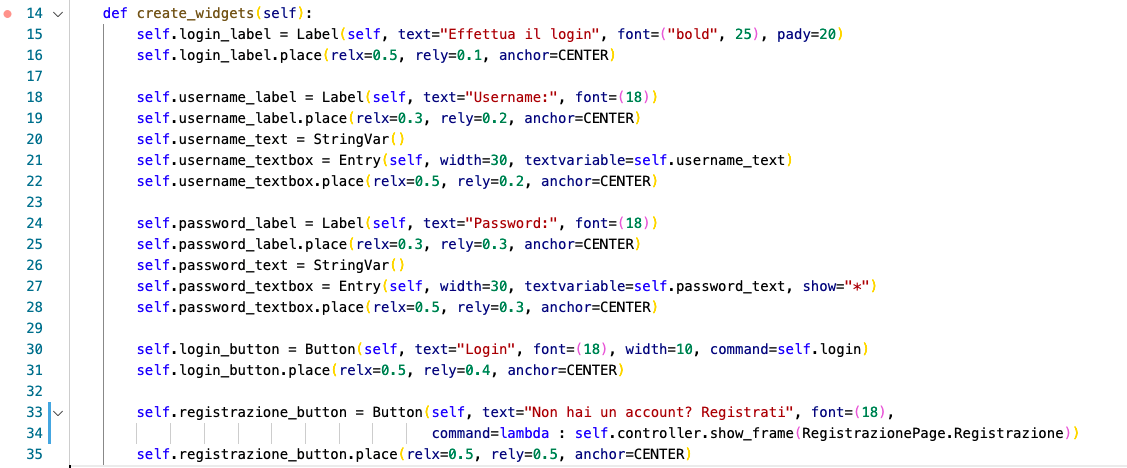
\includegraphics[width=1.0\textwidth]{immagini/createwidgets.png}
\caption{Metodo create\_widgets() di LoginPage \cite{codice}}
\label{fig:createwidgets}
\end{figure}

Inoltre l'attributo \verb+controller+ è di tipo MainPage e si riferisce all'oggetto MainPage che ha creato quello specifico Frame, il quale sarà utilizzato per chiamare il metodo \verb+show_frame()+ per cambiare schermata.

La classe \textbf{MainPage} ha lo scopo di gestire le schermate e le loro transizioni, e lo fa con il metodo \verb+show_frame(Frame)+, in particolare questa classe ha una lista di oggetti Frame che rappresentano tutte le varie schermate dell'applicazione, e quando questo metodo viene invocato esso mostra il Frame che gli è stato passato come parametro mentre elimina tutti gli altri, in questo modo viene cambiata la schermata mostrata a video.

\section{Database}
La classe che gestisce la connessione al database è \textbf{DB}, e quando viene istanziata si connette al database usando i parametri definiti in un file di configurazione che deve essere presente e avere il seguente formato:
\newpage
\begin{verbatim}
host=localhost
database=nomedb
user=nomeuser
password=password
\end{verbatim}
La classe DB si collegherà a questo database e, se non sono già presenti, creerà le seguenti tabelle:
\begin{itemize}
\item \textbf{users}: rappresenta tutti gli utenti registrati all'applicazione, i quali sono descritti da diversi attributi:
\begin{itemize}
\item username: è la primary key e rappresenta quindi l'identificatore unico di ogni utente, viene usato per fare il login
\item nome
\item cognome
\item password
\end{itemize}
\item \textbf{companies}: è la tabella delle aziende disponibili nell'applicazione, descritte dagli attributi:
\begin{itemize}
\item nome: è la primary key, quindi è unica per ogni azienda ed è il nome legale dell'azienda
\item market: rappresenta il settore di mercato in cui l'azienda opera
\item total\_investment: è il totale in dollari di investimenti che l'azienda ha ricevuto nel corso della sua vita
\item funding\_rounds: è il numero di investimenti totali ricevuti, cioè quante volte si è investito nella azienda a prescindere dalla somma di denaro
\item founded\_at: rappresenta la data in cui è stata fondata
\item first\_funding\_at: rappresenta la data in cui ha ricevuto il primo investimento, questo attributo servirà per calcolare dei dati derivati per l'algoritmo di machine learning per la predizione dell'andamento (si veda \ref{subsubsec:class})
\item last\_funding\_at: rappresenta la data dell'ultimo investimento ricevuto, e come l'attributo \textit{first\_funding\_at} serve per calcolare dei dati derivati (si veda \ref{subsubsec:class})
\end{itemize}
\item \textbf{interested}: è la tabella che descrive gli interessi di tutti gli utenti, cioè quali aziende sono nei preferiti di ogni utente, gli attributi sono due e sono delle foreign key che si riferiscono alle entità user e company:
\begin{itemize}
\item username: primary key dell'utente
\item nome: primary key dell'azienda che l'utente descritto dallo username ha inserito nei preferiti
\end{itemize}
\end{itemize}

La classe DB ha dei metodi per la lettura, scrittura, modifica e eliminazione di queste tabelle, grazie ai quali le classi che rappresentano le schermate possono agire sul database per leggere i dati o effettuare delle modifiche. In questo modo tutta la complessità dell'accesso al database è incapsulata nella classe DB e le altre classi devono solo interagire con l'interfaccia che essa espone. Per lo sviluppo dell'applicazione è stato deciso di usare \textbf{MySQL} come DBMS e farlo girare in locale, ma in caso di modifica del DBMS basterà modificare la classe DB.

Tutte le classi che rappresentano delle schermate interagiscono con il database tramite la classe DB, tranne la classe Company. La classe Login controlla che esista l'utente e che la password inserita dall'utente in fase di accesso sia corretta, altrimenti mostrerà un messaggio di errore. La classe Registrazione controlla che lo username inserito dall'utente non esista già nel database, e nel caso non esista e gli attributi che descrivono l'utente siano stati inseriti nel modo corretto, registra il nuovo utente aggiungendolo alla tabella \textit{users}. La classe CreateCompany esegue la registrazione analoga a quella fatta dalla classe Registrazione ma per le aziende, quindi accedendo alla tabella \textit{companies}. La classe Profilo accede al database per aggiornare i dati modificati dall'utente.  Infine la classe Home accede al database in caso l'utente effettui una ricerca, quindi eseguirà una lettura nella tabella \textit{companies}, se esiste mostra l'azienda cercata altrimenti mostrerà un messaggio che inviterà l'utente ad aggiungere l'azienda non presente.

\section{Integrazione con PredictionIO}
La classe \textbf{Predictor} gestisce la parte di machine learning e fornisce quindi l'interfaccia con cui accedere agli engines di PredictionIO, manderà le query per fare una richiesta ai modelli e riceverà le risposte. Le richieste e le risposte saranno in un certo formato, quindi questa classe ha anche il compito di convertirle nelle varie forme richieste. I metodi principali della classe Predictor sono:
\begin{itemize}
\item \verb+predict_company(nome)+: ha il compito di mandare la richiesta di predire l'andamento futuro dell'azienda passata come parametro all'engine che implementa il modello di classificazione, per farlo deve accedere al database per leggere tutti gli attributi riferiti a quell'azienda.
\item \verb+transform_features(features)+: è il metodo tramite il quale \\ \verb+predict_company()+ converte gli attributi nel formato corretto per l'engine di PredictionIO, gli attributi da convertire sono passati come parametro sotto forma di lista Python. 
\item \verb+predict_consigliati(username)+: è il metodo che interagisce con l'engine che implementa il modello di raccomandazione, esegue una richiesta per avere 30 aziende consigliate all'utente passato come parametro.
\item \verb+insert_consigliato(username, nome)+: quando un utente salva nei preferiti un'azienda questo metodo invia all'event server questo evento, di tipo "interested", che descrive l'interesse dell'utente \textit{username} per l'azienda \textit{nome}. L'evento inviato sarà relativo al modello di raccomandazione, in questo modo l'engine potrà continuare il suo addestramento e fornire consigli più precisi.
\item \verb+insert_nonconsigliato(username, nome)+: è il metodo duale di \\ \verb+insert_consigliato()+, però manda un evento di tipo "not interested", cioè quando l'utente \textit{username} toglie dai preferiti l'azienda \textit{nome}, il che significa che non è più interessato.
\end{itemize}

Per interagire con gli engines la classe Predictor sfrutta le API di PredictionIO per Python, importando il modulo \verb+predictionio+ si potrà istanziare degli oggetti di tipo \verb+EngineClient+ e \verb+EventClient+, i primi per comunicare con gli engine, mandare richieste e ricevere risposte, mentre i secondi per mandare dati sotto forma di eventi all'event server. Di seguito due esempi di utilizzo:
\begin{verbatim}
import predictionio
engine_client = predictionio.EngineClient(url="http://localhost:8000")
event_client = predictionio.EventClient(access_key="access_key", 
 url="http://localhost:7070")

result = engine_client.send_query(query)

event_client.create_event(event="interested", entity_type="user", 
 entity_id=username, target_entity_type="company",
 target_entity_id=nome)
\end{verbatim}

La classe Predictor utilizza un oggetto di tipo \verb+EventClient+ per comunicare con l'event server e distinguerà gli engine passando come parametro le diverse access key, mentre utilizza due oggetti di tipo \verb+EngineClient+, ognuno istanziato per un solo engine.

\subsection{Formato delle richieste e risposte}
Le richieste agli engines devono essere in un certo formato per poter essere comprese, e a loro volta le risposte avranno lo stesso formato, la classe Predictor effettua le dovute conversioni. Il formato è il JSON, in particolare in Python viene usata la struttura dati \textit{dizionario}, cioè un insieme di coppie chiave-valore. 

Nel caso del modello di classificazione il metodo \verb+send_query()+ dell'oggetto \verb+EngineClient+ visto sopra accetta come parametro un dizionario, che avrà come chiavi i nomi delle features accettate dal modello, e come valori i corrispondenti valori delle features. Il risultato che restituisce sarà a sua volta un dizionario con il valore predetto della variabile target specificata nel modello. La trasformazione delle features in un dizionario la effettua il metodo \verb+transform_features()+ della classe Predictor.

Nel modello di raccomandazione il metodo \verb+send_query()+ accetta sempre un dizionario, ma in questo caso rappresenterà lo username dell'utente per il quale vogliamo le aziende raccomandate e il numero delle aziende richieste. Il risultato restituito sarà anch'esso un dizionario che avrà come valore una lista di nomi di aziende predette.

\subsection{Implementazione degli engines di PredictionIO}\label{subsec:impl}
Per lo sviluppo di questo progetto ho implementato due engines di PredictionIO:
\subsubsection{Classificazione}\label{subsubsec:class}
Per il task di previsione dell'andamento futuro delle aziende, l'algoritmo scelto è il RandomForest, un algoritmo di ensemble che sfrutta un insieme di Decision Tree per la previsione. PredictionIO ha a disposizione un template di un engine che implementa questo algoritmo, quindi è necessario solamente modificare alcune parti per adattarlo al problema specifico. In particolare nella componente di Data Source sono state modificate le features e la variabile target che il modello accetta:
\begin{itemize}
\item \textbf{market}: l'attributo di un'azienda che descrive il settore di mercato in cui opera. Questa feature non ha un valore numerico ma è una stringa, per questo motivo viene categorizzata con dei valori numerici per i primi 20 valori più frequenti di \textit{market}, i restanti valori verranno categorizzati come valore "Altro".
\item \textbf{total\_investment}: totale in dollari di investimenti che l'azienda ha ricevuto.
\item \textbf{funding\_rounds}: numero di investimenti totali ricevuti, cioè quante volte si è investito nella azienda a prescindere dalla somma di denaro.
\item \textbf{age\_first\_funding}: questo è un dato derivato che viene calcolato facendo la differenza tra la data in cui l'azienda ha ricevuto il primo investimento e la data in cui l'azienda è stata fondata, in questo modo si ottiene "l'età" in giorni dell'azienda al suo primo investimento. Questo dato viene calcolato dalla classe Predictor nel momento in cui effettua una richiesta all'engine.
\item \textbf{age\_last\_funding}: è un altro dato derivato che viene calcolato in modo analogo al dato age\_first\_funding ma in questo caso viene usata la data dell'ultimo investimento ricevuto, ottenendo così "l'età" in giorni che l'azienda aveva al suo ultimo investimento.
\item \textbf{status}: questa è la variabile target e rappresenta lo stato in cui si trova l'azienda anni dopo rispetto all'anno a cui sono riferiti i dati delle features, lo stato può assumere tre diversi valori: \textbf{operating}, cioè l'azienda non subisce variazioni particolari e continua ad operare; \textbf{closed} se l'azienda è fallita; \textbf{acquired} se l'azienda è stata acquisita da un'azienda più grande.
\end{itemize}

Il modello sarà quindi addestrato per predire lo stato dell'azienda in futuro partendo dai dati descritti dalle features, se lo stato predetto sarà \textit{operating} non verrà dato nessun consiglio particolare, se sarà \textit{closed} verrà consigliato di non investire mentre se sarà \textit{acquired} verrà consigliato di investire.

L'addestramento è stato fatto partendo dal dataset "investment\_VC.csv" \cite{dataset} preso dal sito web Kaggle.com, che rappresenta diverse aziende operanti in tutto il mondo con numerose features, ne è stata fatta una breve analisi selezionandone solo le più rilevanti per ottenere delle buone performance mantenendo però un numero di features limitato. Le aziende presenti in questo dataset sono quelle presenti di default nel database dell'applicazione.

Infine è stato fatto il deploy dell'engine sulla macchina locale su cui girerà anche l'applicazione, in particolare alla porta 8000, in questo modo sarà accessibile all'indirizzo \textit{http://localhost:8000}.

\subsubsection{Raccomandazione}\label{subsubsec:racc}
Per il task di raccomandazione di aziende sulla base delle preferenze degli utenti è stato scelto un algoritmo della libreria MLLib di Apache Spark, l'algoritmo ALS (Alternating Least Squares), questo algoritmo è anch'esso implementato in un engine template di PredictionIO, quindi partendo da questo template è stato necessario effettuare alcune modifiche per adattarlo al caso specifico. 

Sono stati creati due tipi di entità: \textbf{user} e \textbf{company}, rappresentative rispettivamente degli utenti dell'applicazione e delle aziende. Inoltre è necessario rappresentare due tipi di evento: quando un utente inserisce tra i preferiti un'azienda, evento di tipo \textbf{interested}; e quando un utente toglie dalla lista dei preferiti un'azienda, evento di tipo \textbf{not interested}. Inoltre il template di partenza consentiva a degli utenti di assegnare delle valutazioni a degli item con un punteggio, entro un certo range di valori, in questo caso invece è necessario avere solamente due tipi di "valutazioni": una che rappresenti l'inserimento nei preferiti di un'azienda, e l'altra che rappresenti l'eliminazione di un'azienda dai preferiti. Per fare ciò sono stati mappati i due tipi di evento con due valutazioni con un punteggio, in questo modo sono possibili solamente due tipi di punteggio, uno che rappresenta l'evento \textit{interested}, l'altro \textit{not interested}, il tutto viene fatto in automatico dall'engine e l'applicazione, e tanto meno l'utente, non vedranno niente.

Modificando l'engine come spiegato sopra è possibile mandare all'event server, specificando l'access key relativa all'engine che implementa il modello di raccomandazione, degli eventi dei due tipi specificati e il modello sarà in grado di addestrarsi su questi dati e fornire poi una lista di aziende consigliate per ogni utente. Il modello può essere continuamente addestrato anche durante l'utilizzo, man mano che gli utenti mandano dati all'event server, infatti ogni volta che un utente inserisce o toglie dalla lista dei preferiti un'azienda viene mandato in automatico l'evento all'event server. In questo modo basterà riaddestrare il modello con il comando \verb+pio-docker train+ per aggiornare l'engine con i nuovi dati.

Anche per questo engine è stato fatto il deploy sulla macchina locale, stavolta alla porta 8001 con il comando \verb+pio-docker deploy --port 8001+, sarà quindi accessibile all'indirizzo \textit{http://localhost:8001}.

Avendo gli engine disponibili come servizi web alle porte 8000 e 8001 sulla macchina locale, i due oggetti EngineClient con cui la classe Predictor comunicherà con i modelli saranno:
\begin{verbatim}
engine_client_classificazione = predictionio.EngineClient(
	url="http://localhost:8000")
engine_client_raccomandazione = predictionio.EngineClient(
	url="http://localhost:8001")
\end{verbatim}

Nel caso si volesse implementare gli engine su una macchina server dedicata e rendere accessibili i modelli come servizi web anche dall'esterno, lato applicazione basterà modificare le definizioni dei due oggetti EngineClient mettendo come parametro \textit{url} l'indirizzo dei servizi web.
\chapter{Conclusione}\label{c:conclusione}

Lo svolgimento di questo progetto mi ha permesso di approfondire l'argomento del machine learning, non tanto dal punto di vista tecnico ma più dal punto di vista della funzione che esso sta assumendo nel mondo informatico odierno, infatti, nelle sue numerose varianti, è ormai parte integrante di ogni applicazione, che sia web o mobile. Per questo ho deciso di focalizzarmi più sull'integrazione degli algoritmi di machine learning con le applicazioni e su come queste due branche dell'informatica effettivamente interagiscono. Il progetto Apache PredictionIO è molto rappresentativo di questo aspetto, infatti consente di isolare la complessità del machine learning in moduli, chiamati engines, e lasciare allo sviluppatore solamente il compito di modificare questi engines e integrarli con le loro applicazioni.  Progetti simili consentono la diffusione ancora maggiore del machine learning in quanto lo rendono accessibile a tutti gli sviluppatori e non solo ai data scientist.

Lo studio di PredictionIO mi ha permesso di imparare com'è strutturato un progetto software di grandi dimensioni, studiarne l'architettura e come viene implementato a livello pratico. Infatti con l'implementazione degli engines per la classificazione e la raccomandazione ho imparato a modificare codice già scritto, capendone il significato e la struttura per andarlo a modificare adattandolo alle mie esigenze. In secondo luogo ho potuto costruire, sebbene in  locale, dei servizi web, eseguendone il deploy su diverse porte. Infine installando PredictionIO con Docker ho avuto modo di sfruttare e imparare questo software per la containerizzazione molto utilizzato al giorno d'oggi per i vantaggi che offre, quali la leggerezza e la portabilità.

La seconda parte di questo progetto mi ha permesso inoltre di cimentarmi nello sviluppo di un'applicazione, approfondendo il linguaggio Python applicato alla creazione di applicazioni piuttosto che all'analisi dei dati, usando in modo dettagliato le classi e in generale il paradigma di programmazione orientato agli oggetti. Per lo sviluppo dell'applicazione ho avuto anche l'opportunità di studiare e imparare a usare la libreria grafica di Python, TKinter; approfondire l'interazione del linguaggio con un database come MySQL, sfruttando il modulo relativo; e infine la gestione di un'interfaccia per l'interazione con dei servizi web esterni, implementata nella classe Predictor sfruttando le API di PredictionIO disponibili per Python.

\appendix

\printbibliography[heading=bibintoc]

\end{document}
